\clearpage

\section{Validation du design} \label{sec:Validation-design}
Dans cette section, nous décrirons la procédure de vérification des caractéristiques du projet ainsi que sa validation.

\subsection{Liste de matériel} \label{ssec:Liste-materiel}
\begin{itemize}
	\item \textbf{P1} : Oscilloscope Tektronix RTB2004 ES.SLO2.05.01.11
	\item \textbf{P2} : Multimètre GwInstek GDM-396 ES.SLO2.00.00.94
	\item Carte Mini-Boite-Noire 1924B
\end{itemize}

\subsection{Consommations}
Dans cette section, nous mesurerons les différentes consommations du système. Cette étape est importante pour caractériser le système et déterminer son autonomie.

\subsubsection{Méthode de mesure}
L'objectif est de basculer entre les différents modes (veille, logging...) de la carte et d'en mesurer la consommation. À cet effet, un ampèremètre a été placé en série avec la batterie, comme illustré à la figure \ref{fig:schema-courant}.

\subsubsection{Schéma de mesure}

\begin{figure}[h]
	\centering
	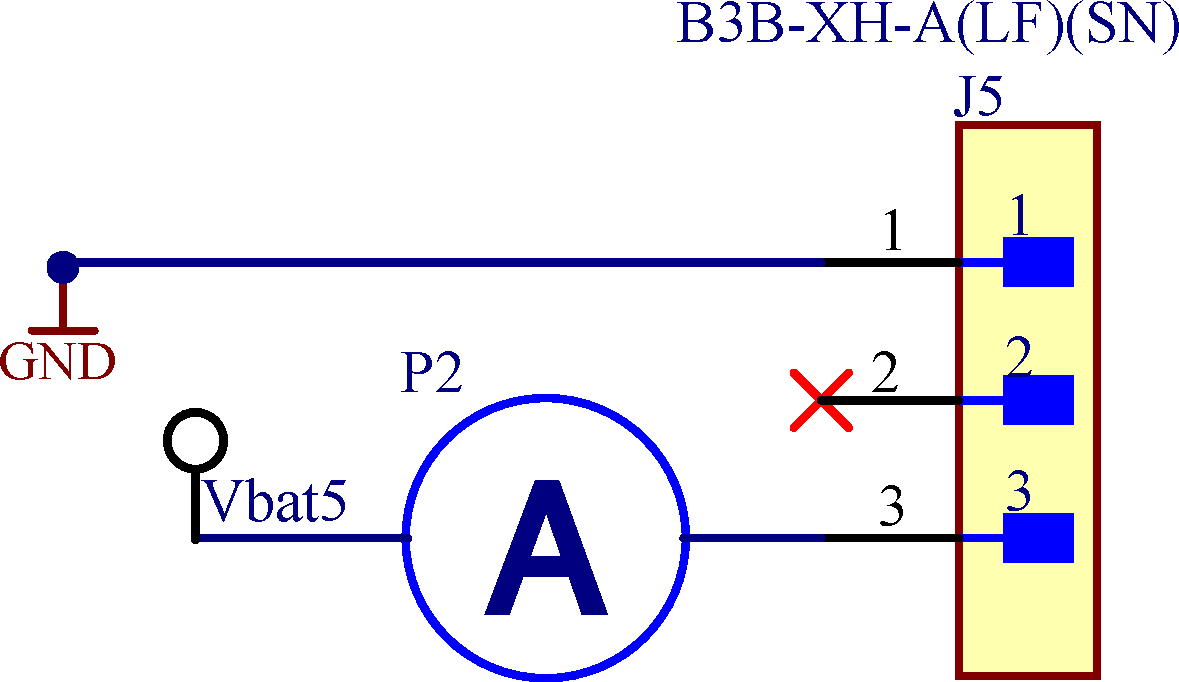
\includegraphics[width=.32\linewidth]{../figures/mesures/schema-courant}
	\caption{Schéma de mesure, courant}
	\label{fig:schema-courant}
	\source{Auteur}
\end{figure}

\subsubsection{Mesures}

\begin{table}[!h]
	\centering
	\resizebox{.78\textwidth}{!}{%
		\begin{tabular}{|c|l|l|c|c|}
			\hline
			\multicolumn{1}{|l|}{Index} & Etat du système & Condition                      & Courant [mA] & Symbol      \\ \hline
			[1]                         & Eteint.         & Mode auto-enclenchement OFF.   & 0.02         & $I_{off}$   \\ \hline
			[2]                         & Veille.         & Est passé par l'état SHUTDOWN. & 4.4          & $I_{sleep}$ \\ \hline
			[3]                         & Veille brutale.\footnotemark & Pas passé par l'état SHUTDOWN. & 9.56         & $I_{ws}$    \\ \hline
			[4]                         & Initialisation. & -                              & 90           & $I_{init}$  \\ \hline
			[5]                         & Logging.        & -                              & 100          & $I_{log}$   \\ \hline
			[6]                         & Shutdown.       & -                              & 83           & $I_{sh}$    \\ \hline
			[7]                         & Communication.  & USB branché.                   & 0            & $I_{usb}$   \\ \hline
		\end{tabular}%
	}
	\caption{Mesure des consommations}
	\label{tab:mes-cons}
	\source{Auteur}
\end{table}

\footnotetext{Lorsque le système a été éteint de façon non-contrôlée (Batterie débranchée).}

Nous pouvons par les mesure de la table \ref{tab:mes-cons} déduire les éléments suivants : 

Où : 

Capacité de la batterie $C = 1600\;mAh$

\begin{tabular}{llll}
	$\bullet$ & Temps de logging &  (Table \ref{tab:mes-cons}-[5]) : & $T_l = \frac{C}{I_{log}} = 16h$. \\
	$\bullet$ & Temps épuisement batterie en veille & (Table \ref{tab:mes-cons}-[2]) : & $T_l = \frac{C}{I_{sleep}} = 364h = 15J$. \\
	$\bullet$ & Temps épuisement en veille brutale & (Table \ref{tab:mes-cons}-[3]) : & $T_l = \frac{C}{I_{ws}} = 167h = 7J$. \\
\end{tabular}

Par conséquent, les caractéristiques d'autonomie de la batterie sont suffisantes pour notre application. 

\paragraph{Proposition de stratégies d'économie d'énergie}
Afin de diminuer la consommation lors du mode veille il existe différentes possibilités :

\noindent\textbf{Débraser la LED de la carte BNO0555 d'adafruit}

\begin{figure}[!h]
	\centering
	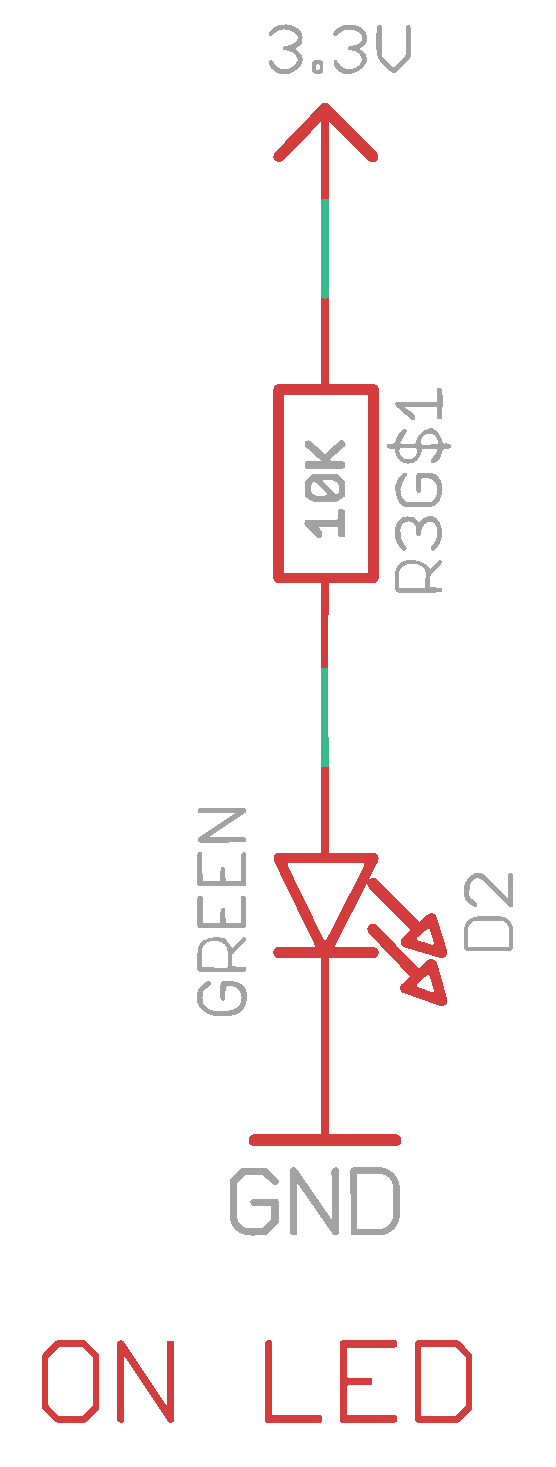
\includegraphics[width=0.15\linewidth]{../figures/mesures/led-imu}
	\caption{Ajout}
	\label{fig:led-imu}
	\source{Schéma de la \href{https://cdn-learn.adafruit.com/assets/assets/000/092/544/original/sensors_BNO055_STEMMA_sch.png?1593120280}{carte BNO055 d'adafruit }}
\end{figure}

\noindent\textbf{Permettre de changer de mode plus facilement} Permettre à l'utilisateur de facilement basculer entre le mode "auto-enclenchement" et "enclenchement manuel" permettrait d'éviter des consommations inutiles.



\subsection{Bus de communications}
Avec le code implémenté dans le microcontrôleur, les différents périphériques fonctionnent correctement et la communication avec les différents bus est opérationnelle. C'est pourquoi, dans cette section, l'objectif principal est de mesurer la qualité et l'intégrité des signaux plutôt que d'analyser les différents protocoles.

\subsubsection{Communication I2C} \label{ssec:Comm-I2C}
\paragraph{Méthode de mesure}
\paragraph{Mesures}

\begin{figure}[!h]
	\centering
	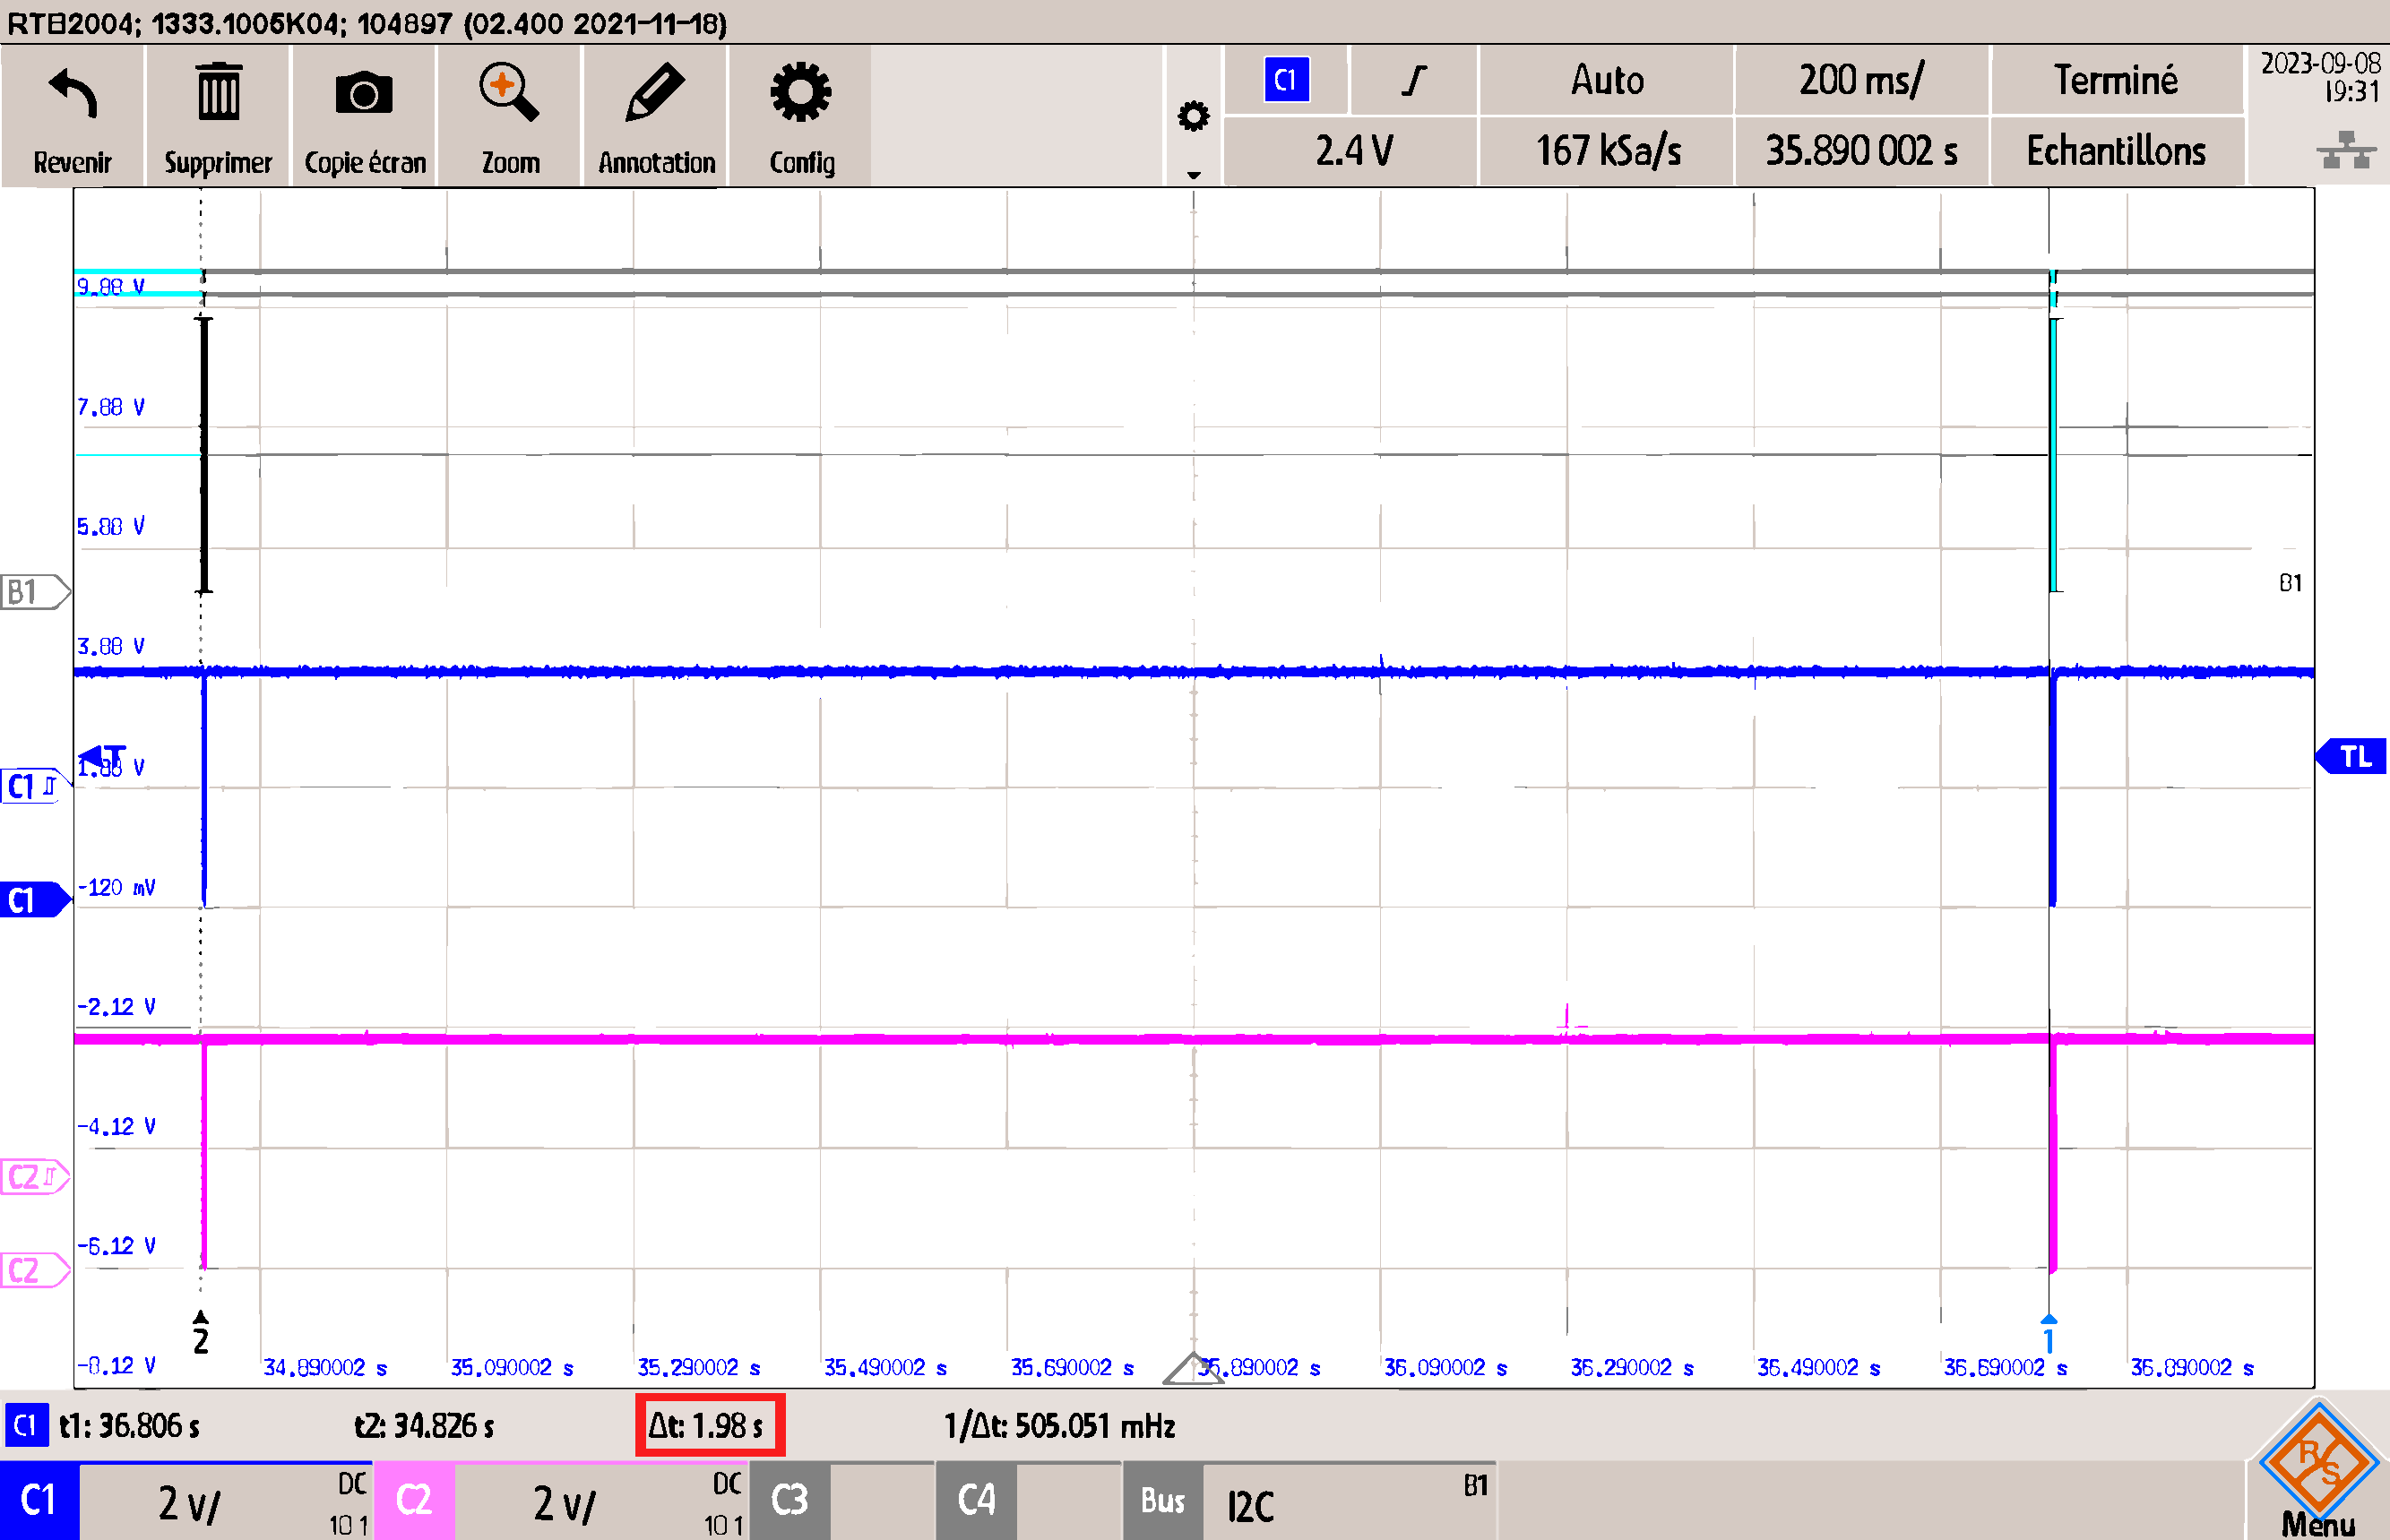
\includegraphics[width=0.7\linewidth]{../figures/mesures/I2C/Intervale-2s}
	\caption{Intervale entre deux mesures, config. 2 secondes.}
	\label{fig:intervale-2s}
	\source{Auteur}
\end{figure}

\begin{figure}[!h]
	\centering
	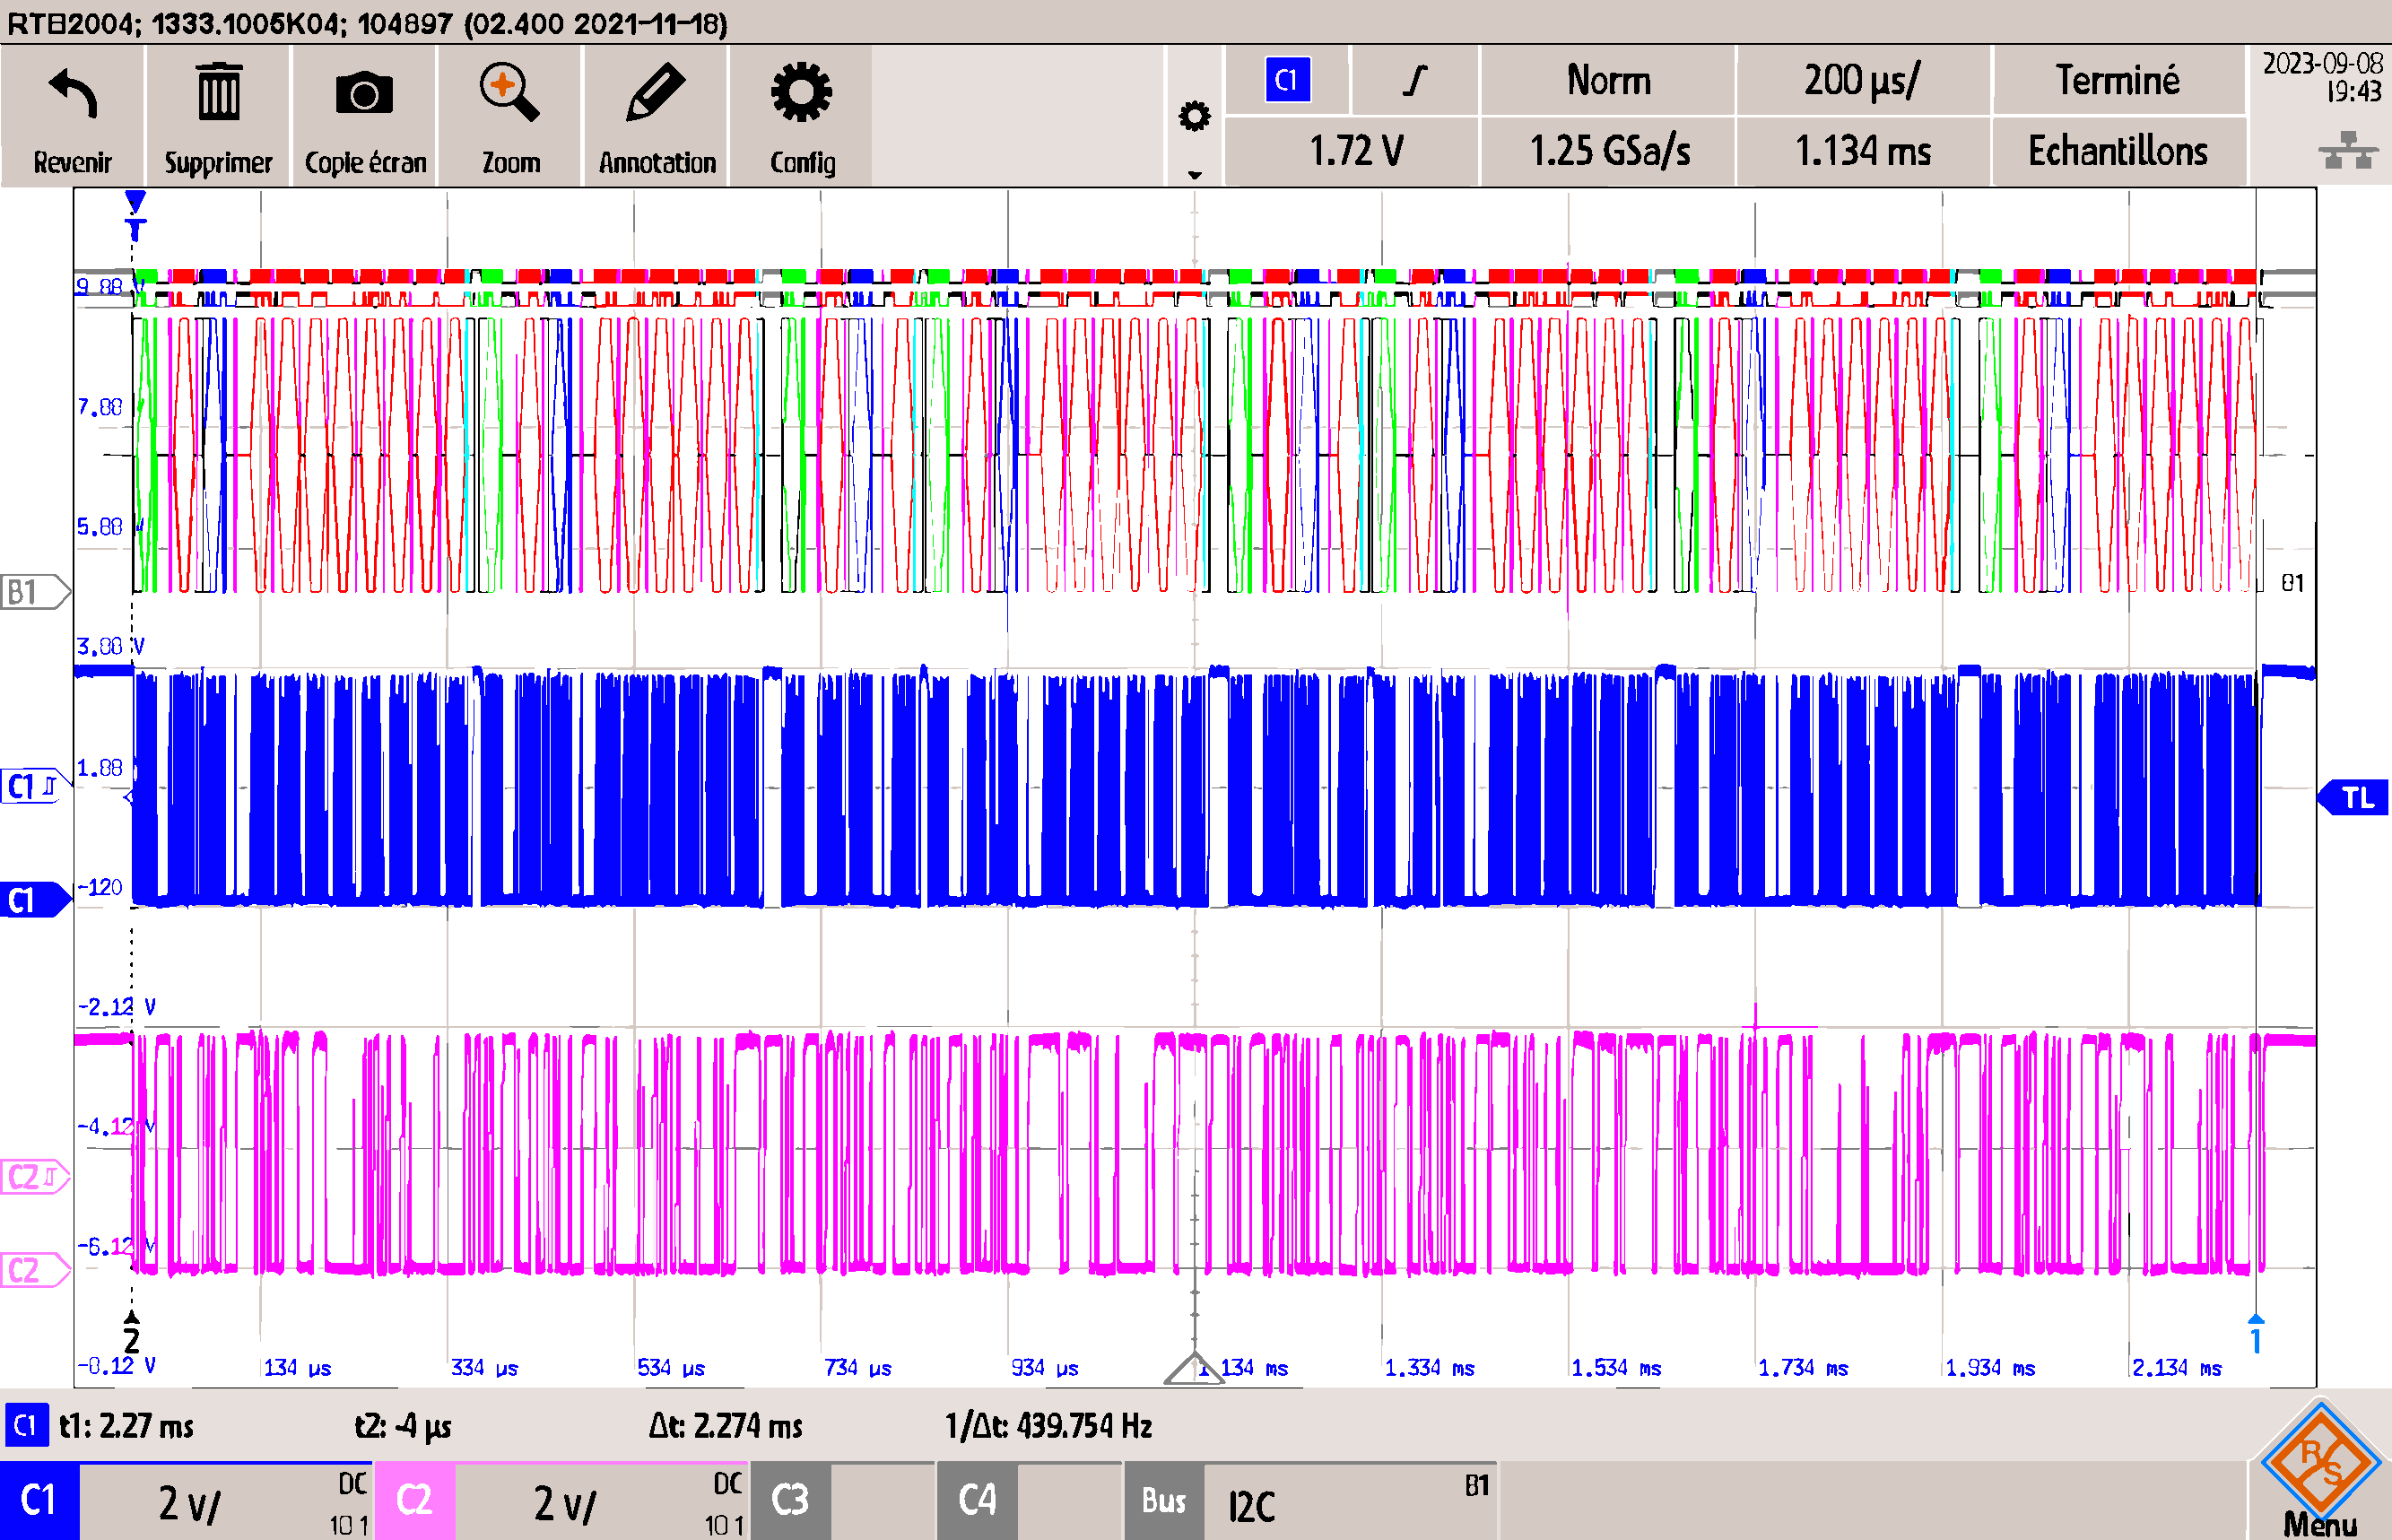
\includegraphics[width=0.7\linewidth]{../figures/mesures/I2C/duree-comm}
	\caption{Durée d'une mesure.}
	\label{fig:duree-comm}
	\source{Auteur}
\end{figure}

\begin{figure}[!h]
	\centering
	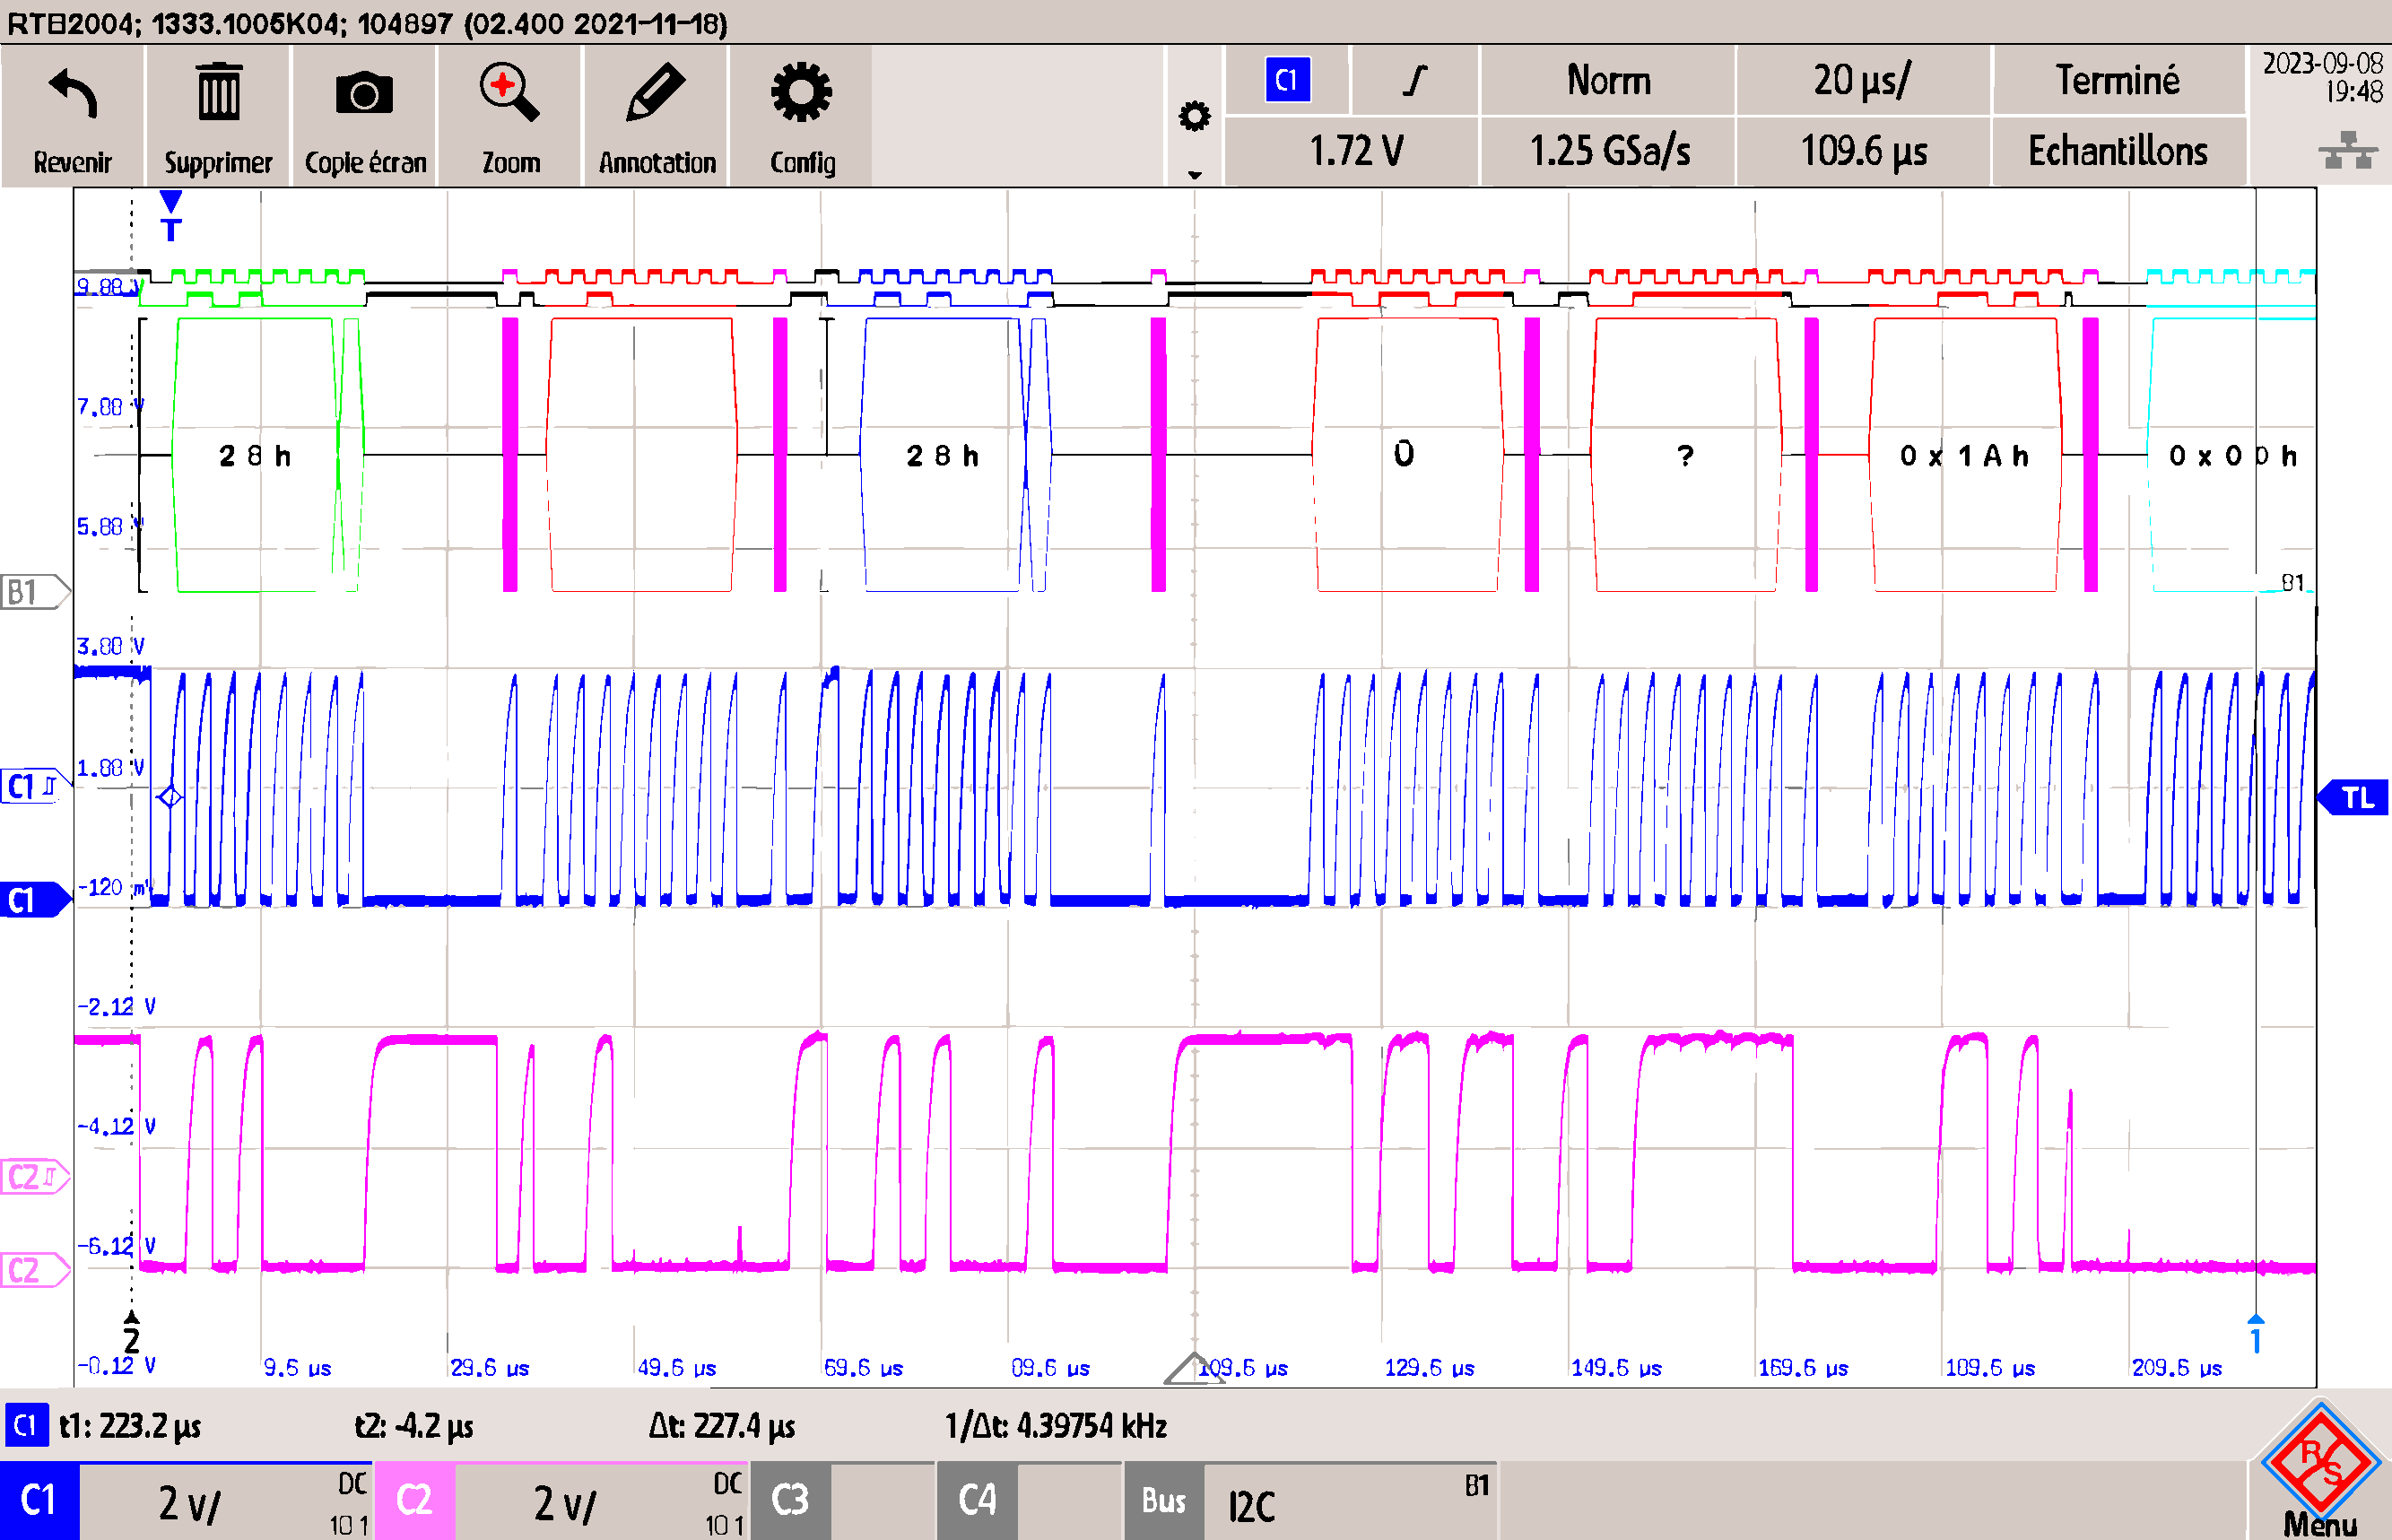
\includegraphics[width=0.7\linewidth]{../figures/mesures/I2C/Tramme-mesure}
	\caption{Début de tramme d'une mesure.}
	\label{fig:tramme-mesure}
	\source{Auteur}
\end{figure}

\subsubsection{Communication UART} \label{ssec:Comm-UART}
\paragraph{Méthode de mesure}
\paragraph{Mesures}

\begin{figure}[!h]
	\centering
	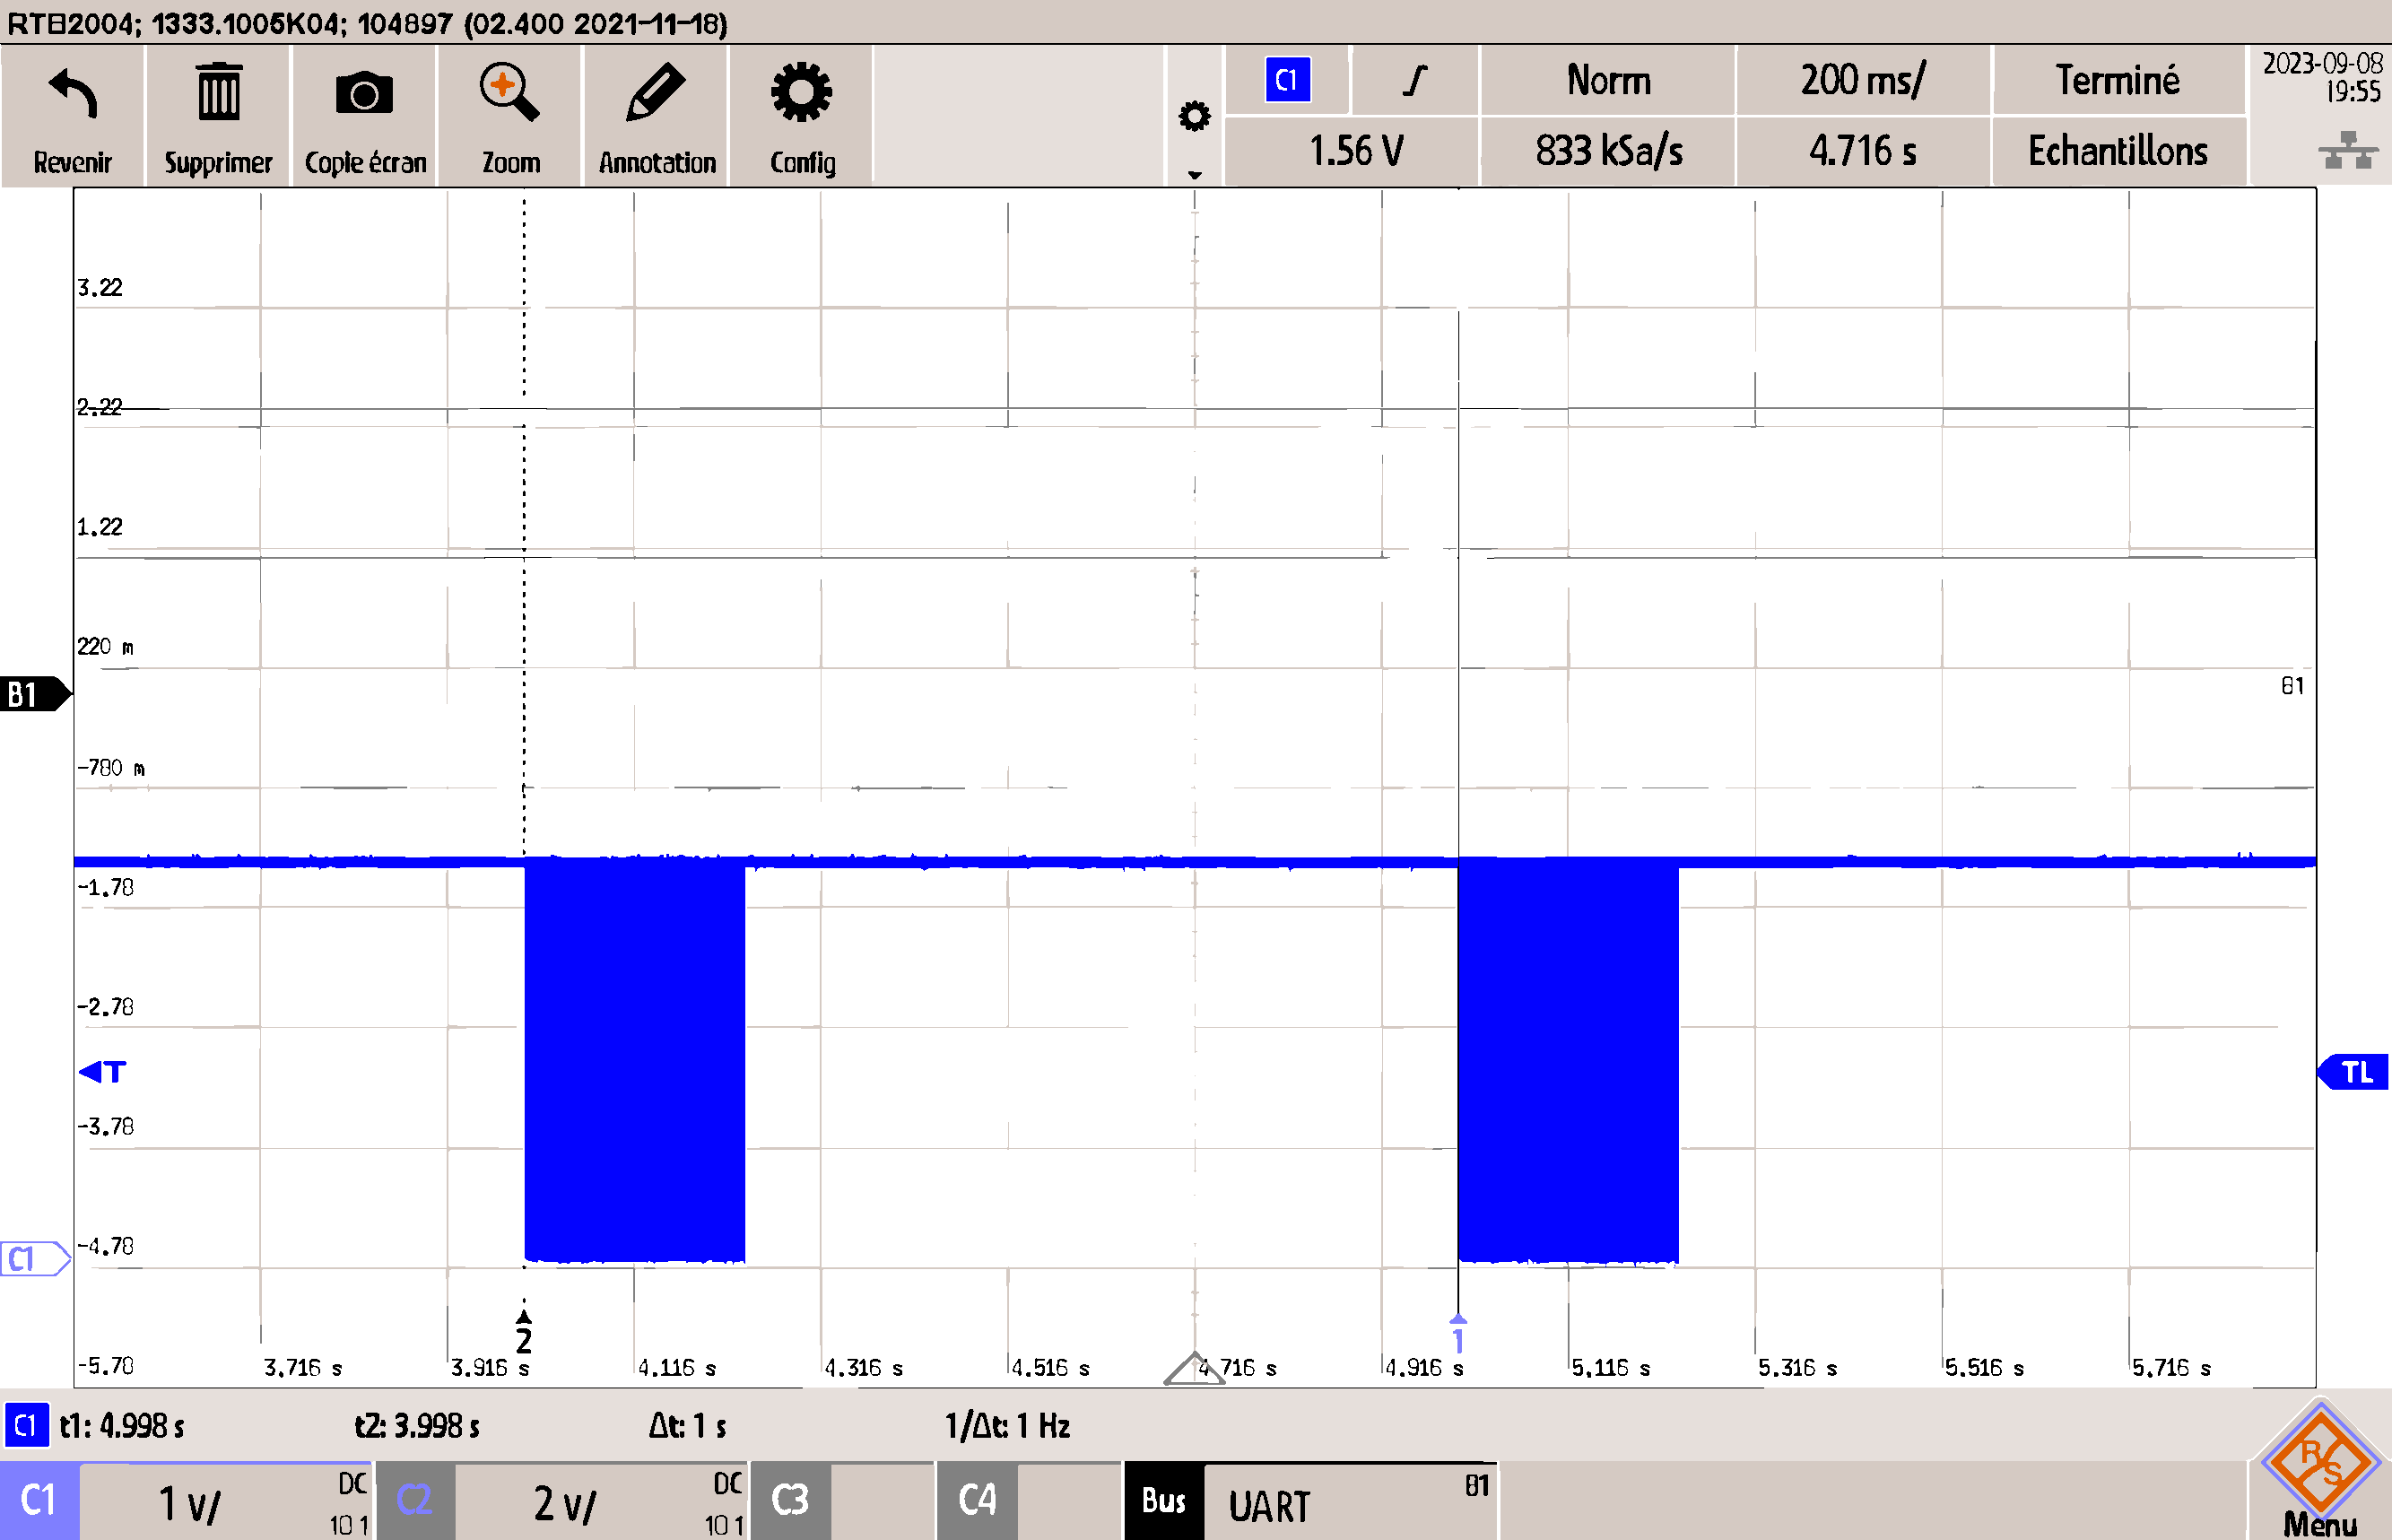
\includegraphics[width=0.7\linewidth]{../figures/mesures/UART/interval-gnss}
	\caption{Intervale entre les données NMEA.}
	\label{fig:interval-gnss}
	\source{Auteur}
\end{figure}

\begin{figure}[!h]
	\centering
	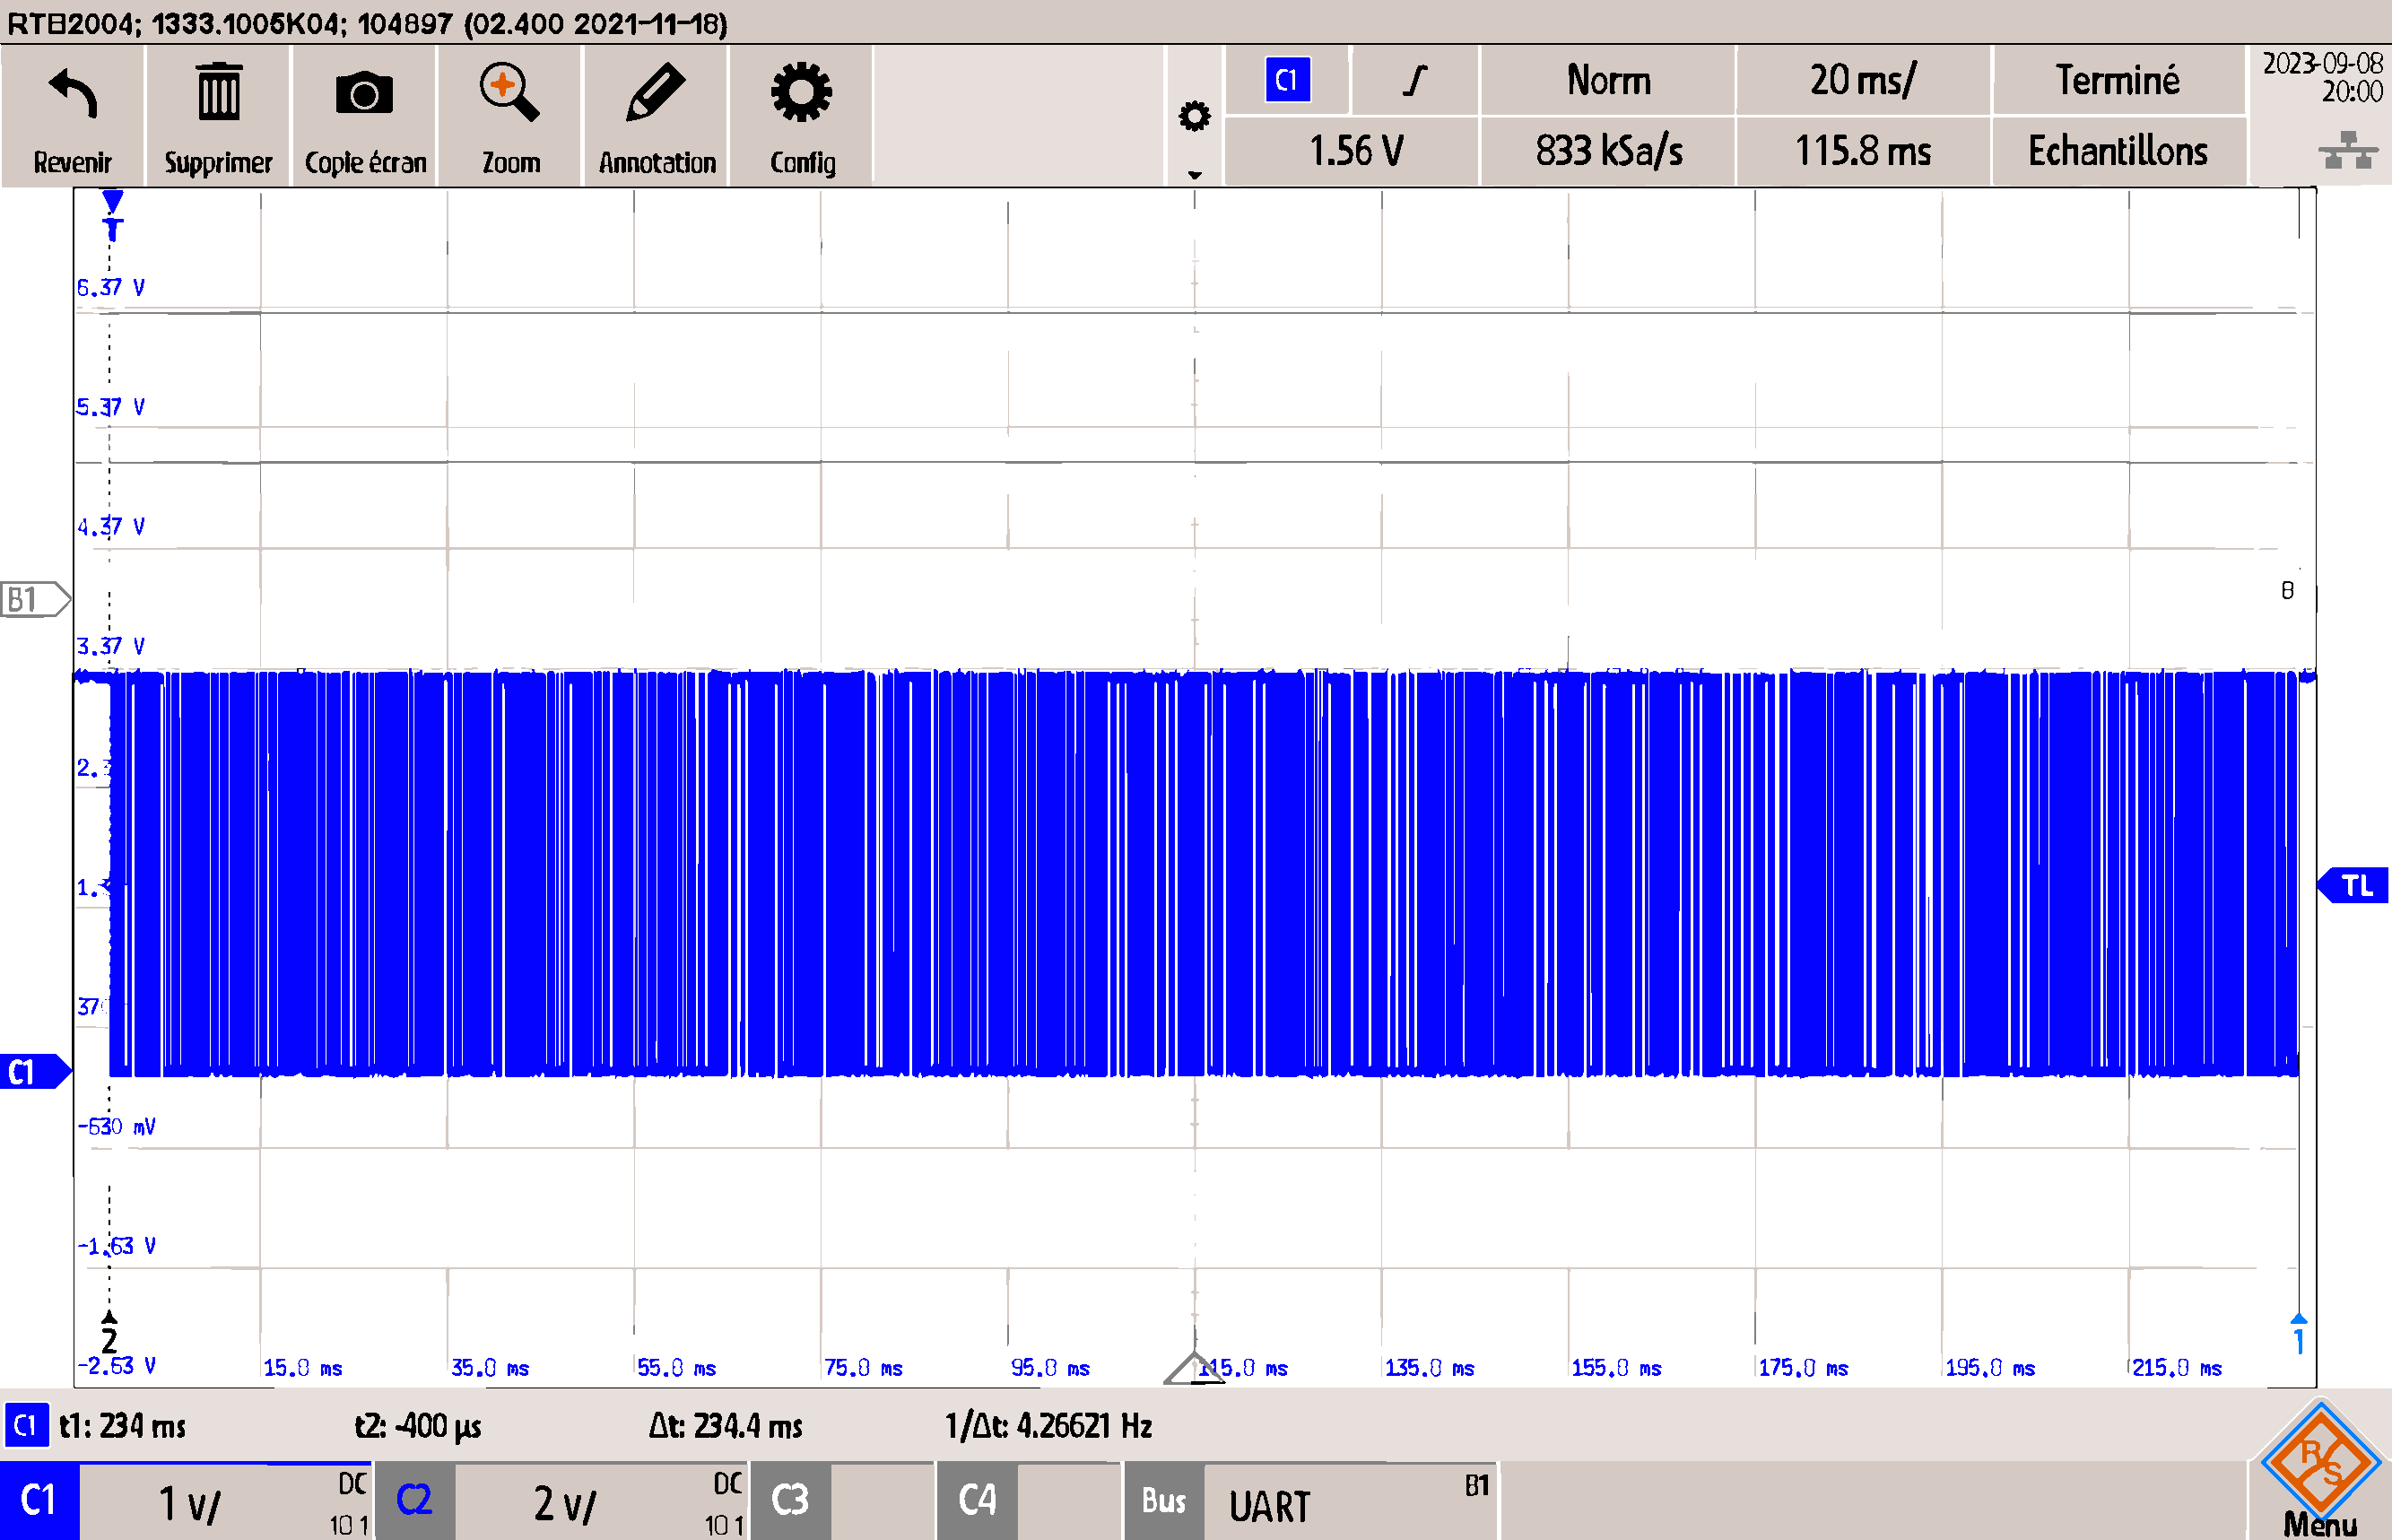
\includegraphics[width=0.7\linewidth]{../figures/mesures/UART/duree-comm-gnss}
	\caption{Durée d'une communication avec le GNSS.}
	\label{fig:duree-comm-gnss}
	\source{Auteur}
\end{figure}

\begin{figure}[!h]
	\centering
	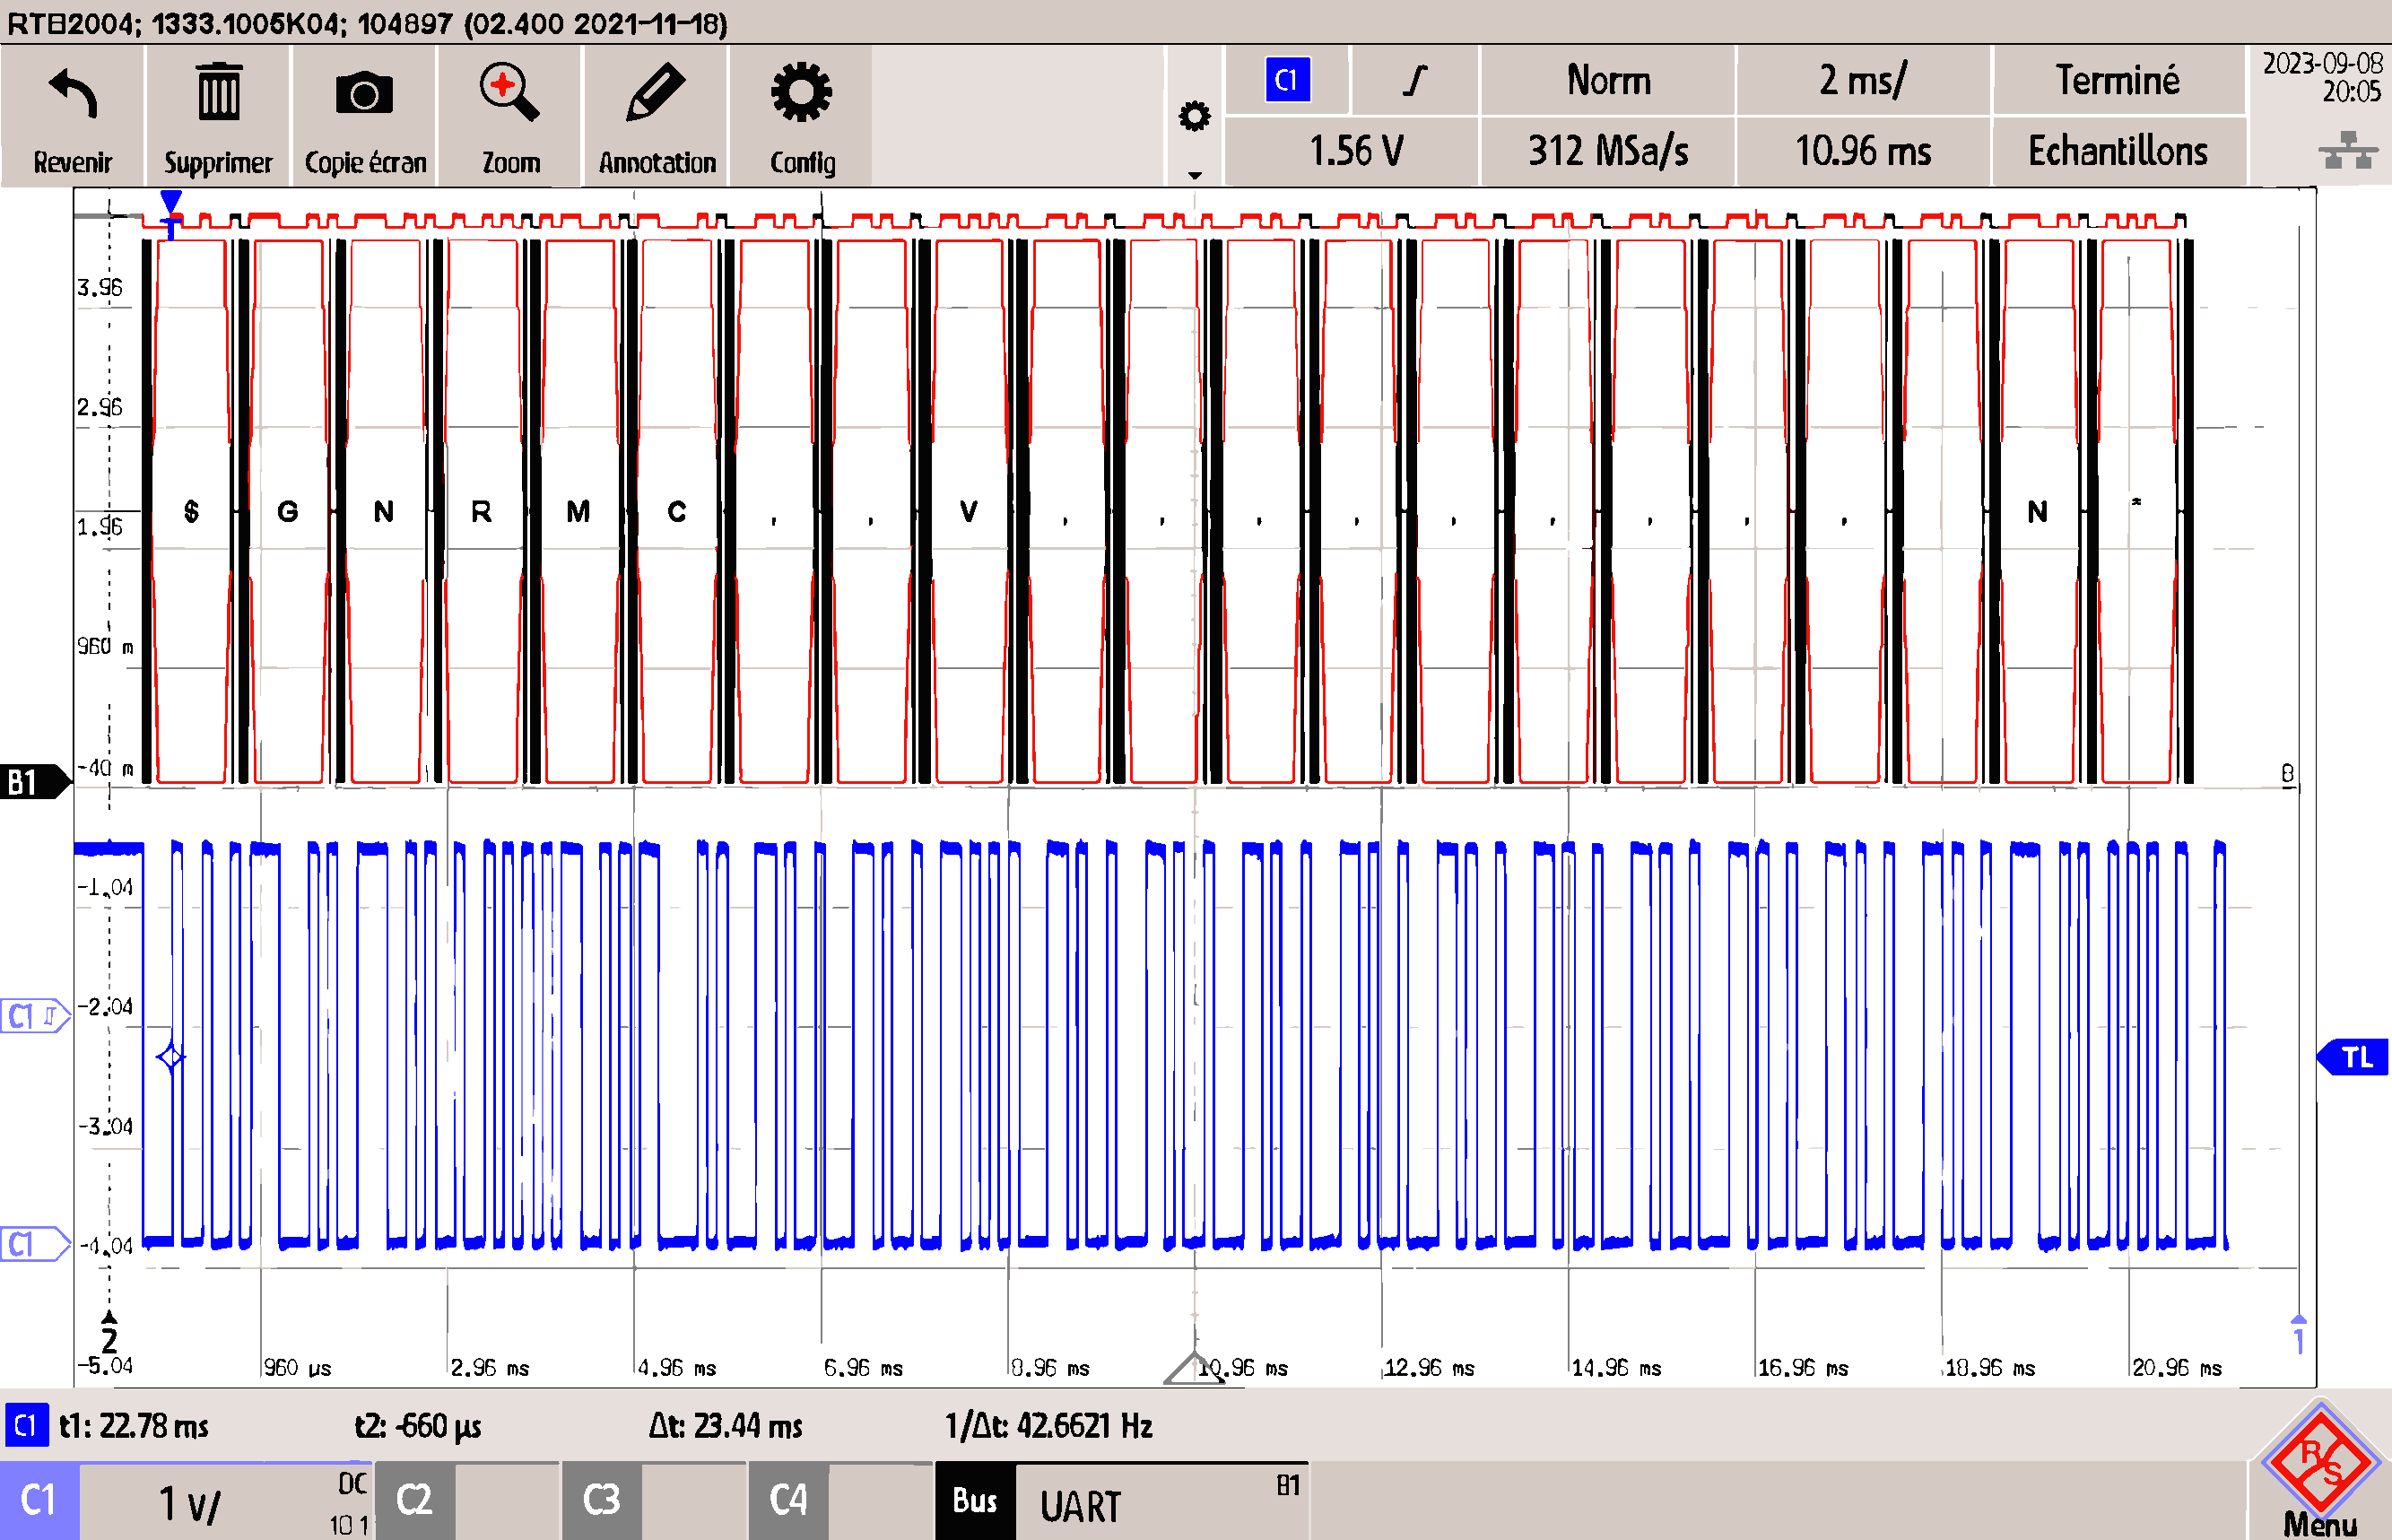
\includegraphics[width=0.7\linewidth]{../figures/mesures/UART/message-NMEA-RMC}
	\caption{Message RMC du protocole NMEA.}
	\label{fig:message-nmea-rmc}
	\source{Auteur}
\end{figure}


\subsubsection{Communication SPI, carte SD} \label{ssec:Comm-SPI}
\paragraph{Méthode de mesure}
\paragraph{Mesures}

\begin{figure}[!h]
	\centering
	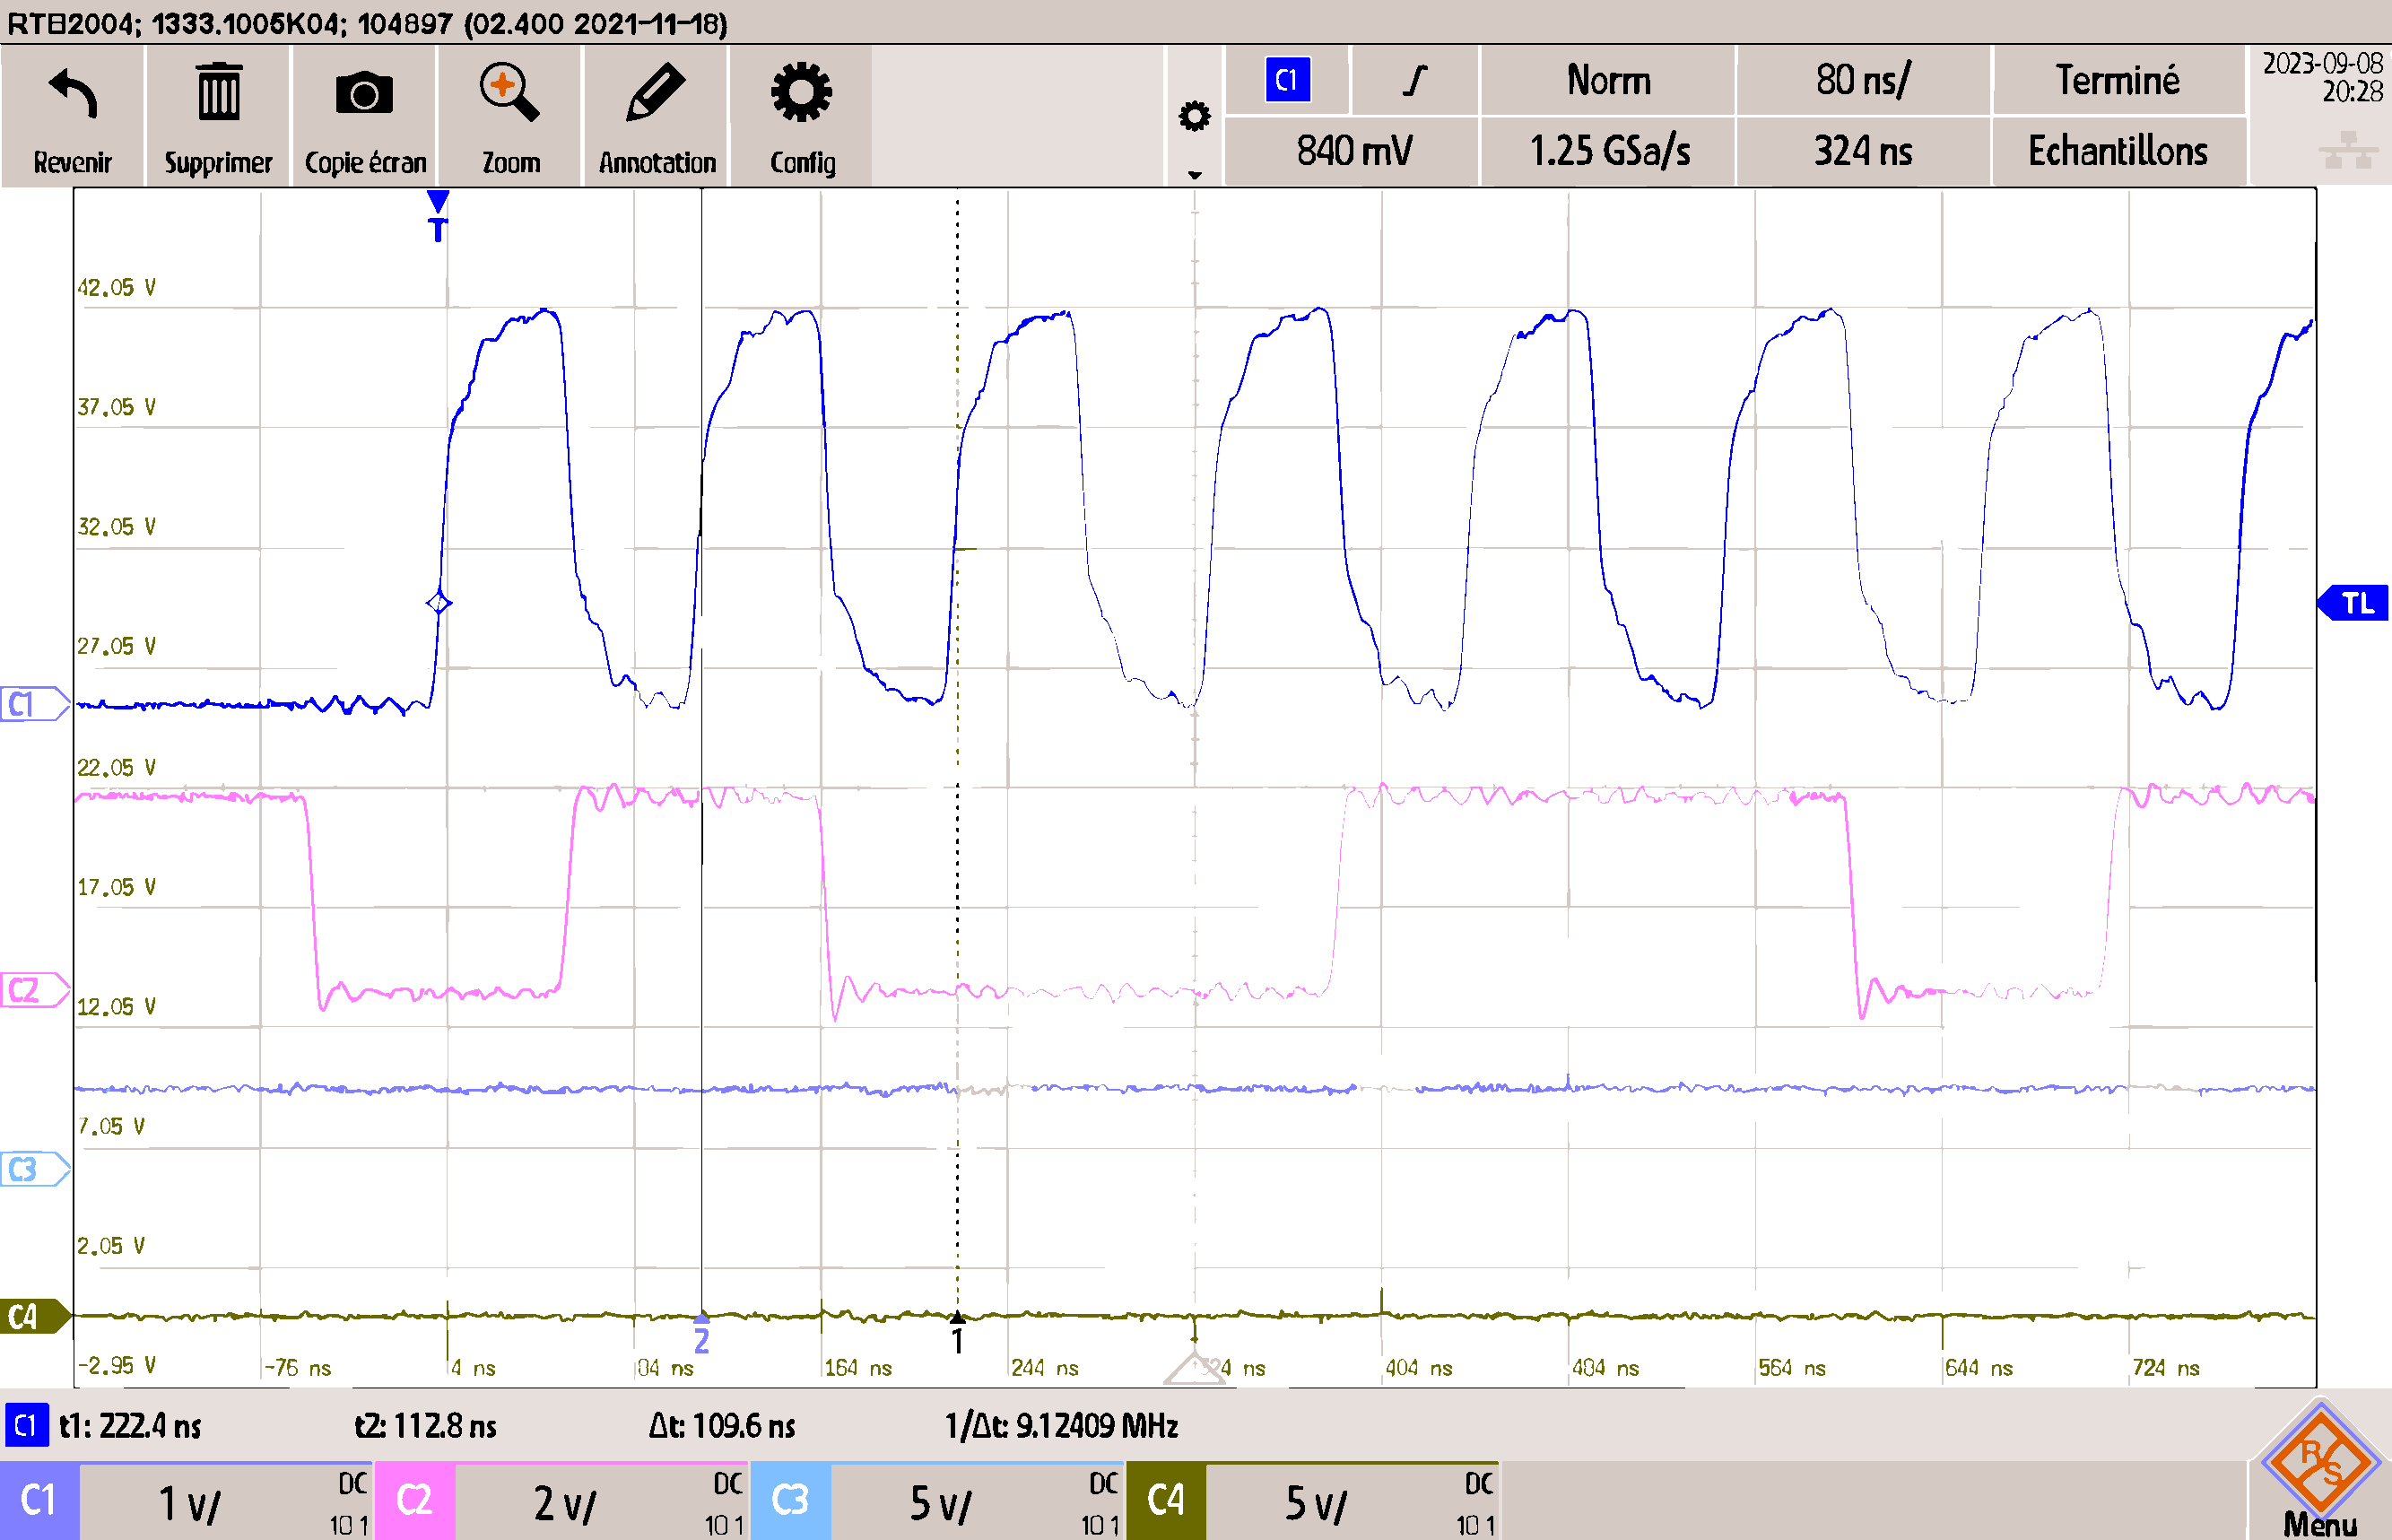
\includegraphics[width=0.7\linewidth]{../figures/mesures/SPI/freq-spi}
	\caption{Mesure fréquence clock SPI.}
	\label{fig:freq-spi}
	\source{Auteur}
\end{figure}



\section{Caractéristiques du produit fini} \label{sec:Carac-finis}